\documentclass[
  dvipdfmx,
  border=2pt
]{standalone}
\usepackage{tikz}
\usetikzlibrary{spath3}
\usetikzlibrary{knots}
\usetikzlibrary{hobby}
\usetikzlibrary{patterns}
\begin{document}
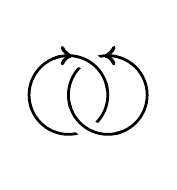
\begin{tikzpicture}[baseline=(current bounding box.center)]
  \begin{knot}[
    % draft mode=crossings,
    flip crossing=2,
    clip width=7,
    every strand/.append style={line width=1pt},
  ]
  \strand (0,0) circle[radius=0.5];
  \strand (0.5,0) circle[radius=0.5];
  \end{knot}
  \draw[->, line width=1.5pt] (0.03, 0.5) -- (0.04, 0.5);
  \draw[<-, line width=1.5pt] (0.46, 0.5) -- (0.47, 0.5);
\end{tikzpicture}
\end{document}